\section{Ejercicios del enunciado}

\subsection{Ejercicio 1}

A lo largo del TP se usan constantes ({\it \#defines\/}), como por ejemplo
en este ejercicio, donde usamos el índice de cada entrada de la {\bf GDT}, declarados
en el archivo {\it defines.h\/}.

Para completar cada entrada se usa la estructura dada por la cátedra sin
ninguna modificación, declarandose descriptores para 2 segmentos de datos y 2 de
código, siendo uno de cada tipo para {\it nivel 0\/} y {\it nivel 3\/}
({\it DPL 0\/} y {\it DPL 3\/}).

% insertar estructura

Se definió un segmento de datos especial para la memoria de video
({\it GDT_VIDEO\/}), el cual se usó solamente en este inciso y se comentó
posteriormente, por ende no se agrega a la GDT (puede apreciarse su código
comentado en el archivo {\it gdt.c\/}).

Luego, se carga la GDT y se salta a modo protegido tal como se vió en las clases
y los ejemplos, seteando el bit {\bf PE} del registro {\bf CR0}, realizando un
{\it jmp\/} con el selector de segmento de código correspondiente y cargando los
selectores de segmento de datos en los registros de segmentos {\it ds, ss, es,
gs\/} y {\it fs\/}.

Todos los segmentos se cargan con la modalidad {\bf flat} y apuntan a la misma
memoria (primeros 500MB). Se apunta la pila del kernel a la dirección
$0\times27000$, especificada por el enunciado, seteando el registro {\bf esp},
consecuentemente, se setea también el registro {\bf ebp}.

Ahora se carga el segmento especial de video y con código assembler se recorre
por medio de 2 ciclos anidados todas las posiciones del segmento, que comienzan
en la posición $0\times B8000$; es decir, se recorre cada posición de la
pantalla pintándola de gris.

De aquí en más se deshabilitó este segmento especial de video y se accede a la
memoria de video por los segmentos de datos. La inicializacion de la pantalla
se realiza en el {\it ejercicio 3\/} con funciones en C.


\subsection{Ejercicio 2}

Para inicializar las entradas de la {\bf IDT} se utilizo la macro {\it IDT_ENTRY\/}
propuesta con una ligera modificacion, se decidió agregar a la misma un
parámetro adicional, que permita especificar el atributo de la entrada,
definidos previamente.
Estas son {\bf TRAP}, la cual indica una trap gate usada para
las excepciones, {\bf INTERRUPT}, usada para interrupciones que solo pueden ser
llamadas por código de privilegio 0, y {\bf USER_INTERRUPT}, que puede ser llamada
por código de usuario también.

\begin{lstlisting}
#define IDT_ENTRY(numero, attribute)
  idt[numero].offset_0_15 = (unsigned short)
                ((unsigned int)(&_isr ## numero) & (unsigned int) 0xFFFF);
  idt[numero].segsel = (unsigned short) (GDT_IDX_ROOT_CODE << 3);
  idt[numero].attr = (unsigned short) attribute;
  idt[numero].offset_16_31 = (unsigned short) (
                (unsigned int)(&_isr ## numero) >> 16 & (unsigned int) 0xFFFF);

#define TRAP      0b1000111100000000
#define INTERRUPT 0b1000111000000000
#define USER_INTERRUPT 0b1110111000000000
\end{lstlisting}

Para la creación de las funciones de las excepciones de procesador se utiliza
otra macro, {\it ISR\/}, esta macro fue adaptada en este ejercicio para que
mostrara un mensaje de error de forma rudimentaria.

\begin{lstlisting}
%macro ISR 2
global _isr%1
  msg%1 db %2, 0
  msg%1_len equ    $ - msg%1
_isr%1:
  mov eax, %1
  imprimir_texto_mp msg%1, msg%1_len, 0x7, 0, 0
  iret
%endmacro
\end{lstlisting}

Cuando se produce una excepción, el descriptor llama a su función asignada
({\it _isrX\/}), la cual, dependiendo del número de interrupción se elige el
mensaje que se imprime por pantalla, esta funcionalidad será aprovechada más
adelante ya que son similares en cuanto a código todas las excepciones en este
tp.

El funcionamiento de la versión final de la macro se detalla mejor en la parte
correspondiente del ejercicio 7, cuando se implementa el verdadero
funcionamiento de las rutinas de atención
de estas excepciones.
% (HABLAR DE LA MACRO DE INTERRUPCIONES)

Una vez inicializada la IDT en el kernel con la macro, como se indica en el
enunciado, se probó a continuación el funcionamiento de varias excepciones.
Esto funcionó correctamente y luego fue comentado para seguir con el trabajo
práctico.



\subsection{Ejercicio 3}

En primer lugar se inicializa la pantalla con la función
{\it screen_inicializar\/} hecha en C.

Esta función utiliza todas funciones de la cátedra, entre ellas
{\it screen_pintar_rect\/}, {\it screen_pintar_linea_h\/},
{\it screen_pintar_puntajes\/}.

Los pasos a realizar por la función son, en primer lugar, pintar toda la
pantalla de gris; luego se pinta una línea negra en la parte superior, donde se
escribirá informacion, por el momento se escribe aquí el nombre del grupo, pero
luego se escribirá la tecla pulsada y el modo {\it debug\/}.
También se pintan los dos sectores de puntajes de los jugadores y se inicializan
los relojes para cada pirata de cada jugador. Todo lo realizado es acorde a las
imágenes del mapa sugerido por la cátedra.

\begin{center}
\includegraphics[width=0.7\textwidth]{imagenes/mapa1.png}

Inicio de la pantalla
\end{center}

Luego se implementó {\it mmu_inicializar_dir_kernel\/} que crea un
{\it page directory\/} para el kernel a partir de la dirección $0\times27000$
como indica el enunciado. En este page directory se crea una primera
{\it page table\/} que se ubica en la posición $0\times28000$, posición
asignada directamente y dicho sea de paso, en este punto, al no estar paginación
aún habilitada, pedir memoria libre no es una buena opción.

La {\it page table\/} se cicla con un incremento de 0 a 1024,
asignando páginas sucesivas, de modo que el esquema de paginación sea
{\bf identity mapping}; y para que ocurra efectivamente, se asigna la page table
en la primera entrada del page directory.
De modo que queda mapeada toda la sección del kernel y su memoria libre.
Como última aclaración, la sección del kernel corresponde al uso de la page
table en su totalidad (1024 entradas).

Finalmente se carga en el {\bf cr3} del kernel la dirección del page directory y
se habilita en el {\bf cr0} el bit de paginación.


\subsection{Ejercicio 4}

Se inicializa el seguimiento de las páginas libres con una variable global
({\it proxima_pagina_libre\/}) que comienza indicando el inicio del sector de
memoria libre, ubicado en la posición $0\times10000$. Con esta variable se
indica el lugar donde se reserva la próxima página pedida y luego se mueve una
posición hacia adelante. Este funcionamiento se implementó en la función
{\it mmu_proxima_pagina_fisica_libre\/}.

Luego se implementaron las funciones {\it mmu_mapear_pagina\/} y
{\it mmu_unmapear_pagina\/}, la primera accede al page directory indicado por
el parámetro {\it cr3\/} y chequea si la page table correspondiente a la
direccion virtual que se pide mapear está presente o no; si no lo está, se
reserva una página libre para alojarla, si lo esta, se apunta a la page table
indicada. En esta tabla setea en la entrada correspondiente a la dirección
virtual, los valores necesarios (base) para mapear a la dirección física, que
corresponden a los primeros 20 bits de la dirección, debido a que las páginas
están alineadas a 4kb. Se pone en presente posteriormente esta la entrada de la
página.

Finalmente se limpia el cache de páginas accedidas. Se agregó además un
parámetro adicional que permite elegir entre mapear la página como
solo lectura ({\bf RO}) o lectura/escritura ({\bf RW}).

Por otra parte, {\it mmu_unmapear_pagina\/} simplemente busca en el page
directory y en la page table correspondiente la entrada que estaba mapeando la
dirección virtual y setea a cero su bit de presente.

La implementación de la función {\it mmu_inicializar_dir_pirata\/} se detalla a
continuación separada por items:

\begin{itemize}
\item Se crea un page directory para el nuevo pirata, pidiendo una página libre, se
setea todo en cero para esta estructura, para evitar que basura de la memoria
mapee páginas no deseadas (de todas formas {\it bochs\/} setea a 0 la memoria
por defecto), y en la primera tabla se apunta a la misma page table que mapea el
kernel, siendo esta la dirección 0x28000, es propicio aclarar que todas las
tareas comparten la misma page table de identity mapping del kernel.

\item Luego se obtiene la direccion física en donde comienza el pirata, que en
el caso del TP, corresponde al puerto del jugador
({\it jugador.puertoX\/} y {\it jugador.puertoY\/}), notar que cambiando el
puerto de la estructura jugador, el pirata puede inicializar de cualquier otra
posición del mapa. Se localiza también con un puntero que se obtiene de
({\it jugador.codigo[tipo_pirata]}) la posición en memoria del codigo
correspondiente al tipo de pirata.

Estos valores de localización del código se asignan al comienzo del juego al
campo {\it codigo\/} de la estructura jugador, son paramétricos y pueden
modificarse si el código de las tareas cambia de ubicación.

\item Con el {\it cr3\/} actual se mapea en la dirección $0\times401000$ el lugar
donde va a ir localizado el código, se copia efectivamente el código a esta
dirección recien mapeada y se pone manualmente en las últimas posiciones de la
pila de la tarea los parámetros {\it x\/} e {\it y\/} necesarios por el código y
una dirección de retorno 0 la cual no va a ser llamada nunca. Finalmente se
desmapea esta dirección $0\times401000$.
Se utiliza la dirección $0\times401000$ porque es una dirección dentro del
segmento de datos que no será mapeada nunca en el TP por ninguna tarea.

\item Se termina por mapear, la dirección $0\times400000$ en el page directory
creado al comienzo de la función, con la posición en memoria a donde se copió el
código de la tarea en los pasos anteriores.
\begin{center}
\includegraphics[width=0.25\textwidth]{imagenes/parametrosTarea.png}

Pila de la tarea con los parámetros cargados
\end{center}

\item En las 4 tablas de páginas siguientes (entrada 2 a 5 inclusive del page
directory) se mapean 4 páginas que se reservaron al inicializar un jugador.

Estas corresponden a indicar las direcciones del mapa que ya son conocidas por
todos los piratas del jugador y se ven actualizadas con cada movimiento de los
piratas exploradores.

Estas 4 tablas de páginas se comparten por todos los piratas de cada jugador, de
esta manera, cada vez que un pirata explorador mapee una nueva posición del mapa
con la función {\it mmu_mapear_pagina\/}, la posición estará mapeada para todos
los piratas del jugador y por ejemplo, un minero se podrá mover a dicha posición.

Por último se exploran las 9 posiciones en la que se crea el pirata, esto es
solo útil para el primer pirata. Al realizarse siempre, las posiciones ya
podrían estar exploradas por piratas previos. Luego se devuelve el page
directory del pirata recién creado. Para realizar esto, se llama a
\hbox{\it game_explorar_posicion(pirata_a_crear, page_directory_del_pirata, puertoX, puertoY, TODO)}
(ver en funciones propias).
\end{itemize}

\subsection{Ejercicio 5}

Se crean las 3 entradas en la IDT para las 3 interrupciones indicadas con:
\begin{lstlisting}
/* Agregamos entrada para interrupcion del clock */
IDT_ENTRY(32, INTERRUPT);
/* Agregamos entrada para interrupcion del teclado */
IDT_ENTRY(33, INTERRUPT);
/* Agregamos entrada para interrupcion de software 0x46 */
IDT_ENTRY(70, USER_INTERRUPT);
\end{lstlisting}

Y las 3 funciones {\it _isr32\/}, {\it _isr_33\/} e {\it _isr70\/}.

Luego se activa el PIC con {\it resetear_pic\/} y {\it habilitar_pic\/}.

En la interrupción del reloj se avisa al PIC que se atendió la interrupción con
{\it fin_intr_pic1} y se realizaba lo pedido en el enunciado, llamándose a
{\it game_tick\/} que actualizaba el reloj del sistema.

% (HABLAR DE LAS 3 INTERRUPCIONES AL FINAL)

En la interrupción del teclado también se llama a {\it fin_intr_pic1\/} y luego
a la función \hbox{\it game_atender_teclado\/}, la cual en primer lugar solo se
encargaba de imprimir en pantalla la tecla usando un switch y los distintos
códigos de teclado.

Se hablará en mayor profundidad de esta y las otras interrupciones cuando se
trate su implementación final.

Finalmente se agrega la interrupcion 0x46, la cual no hacia nada útil. Se
posterga la explicación de su funcionamiento final más adelante cuando es
correctamente implementada.


\subsection{Ejercicio 6}

Se agrega en la GDT un descriptor de {\bf TSS} para la tarea {\it inicial\/},
uno para la tarea {\it idle\/}, 8 para los piratas de jugador A y otras 8 para
los piratas del jugador B. Todos los descriptores poseen {\it DPL 0\/}, de modo
que las tareas de usuario no puedan realizar cambio de contexto y solo puedan
ser realizados por código nivel kernel.

En la función {\it tss_inicializar\/} se configura la TSS de la tarea inicial y
de la tarea idle como se pide, creando estas como variables globales en el
código ({\it tss_inicial} y {\it tss_idle}) y modificando esta estructura con
los valores correspondientes.

Primero para la tss inicial y la idle se asigna su dirección (base) en su
descriptor correspondiente de la GDT y se ponen en 1 el bit de presente.

Se inicializa la estructura de la TSS de la tarea idle, esto significa, setear
la pila local y la pila de nivel 0 ambas en la del kernel ($0\times27000$),
el cr3 actual que es el perteneciente al kernel y los eflags con valor
$0\times202$ que activa las interrupciones enmascarables y el {\bf eip}
apuntando a la posicion $0\times16000$ como pide el enunciado, que corresponde
a la posición donde se ubica el código de la tarea.
Luego se asignan los segmentos de privilegio 0, y el {\it rpl\/} del selector a
0.

Finalmente en un ciclo se inicializan las bases y el bit de presente de todas
los descriptores de TSS de los piratas, que son inicializadas con los valores
posteriormente cuando se lanza un pirata.

Para inicializar las TSS de los piratas, se pide una página para la pila de
nivel 0 y asignando la base y el {\it esp\/} al final de esta página, seteando
su pila local al final de su pagina asignada, pero con el esp 3 posiciones
arriba asumiendo que tiene los dos parámetros y la posición de retorno que se
pasan en la pila.

También se asigna el eip apuntando al principio de la página de código
($0\times400000$). El {\it eflags\/} con valor $0\times202$ y con todos los
segmentos de nivel 3 y RPL 3, es decir, con privilegios de usuario.

Se escribe el código necesario para cargar la tarea inicial como la actual,
cargando el selector de la tarea inicial con {\it ltr\/} e inmediatamente salta
a la tarea idle.

En este punto, modificamos la interrupción $0\times46$, la cual ahora pone en la
pila los parámetros que le pasan y llama a {\it game_syscall_manejar\/}. Esta le
pide al {\it scheduler\/} cual es el jugador actual y el pirata actual y con una
serie de condicionales comprueba cual fue el servicio pedido y llama a
{\it game_syscall_pirata_mover\/}, {\it game_syscall_cavar\/} o
{\it game_syscall_pirata_posicion\/}, si no es ningún caso de los anteriores,
destruye al pirata y devuelve un -1.

\begin{description}
\item[game_syscall_pirata_mover] Esta función chequea en primer lugar que se
haya pedido mover con una dirección válida y hacia una posición válida, en caso
contrario se mata al pirata (se llama a {\it game_pirata_exploto\/}) y se
devuelve -1. Luego puede ocurrir que el pirata sea un {\it explorador\/}, en
cuyo caso mapea las páginas descubiertas en la dirección a la que se mueve
llamando a {\it game_explorar_posicion\/} con el {\it pirata\/}, el {\it cr3\/}
actual, la nueva posición ({\it X,Y\/}) y la dirección como parámetros. En caso
que sea un {\it minero\/}, no mapea ninguna página.

\begin{center}
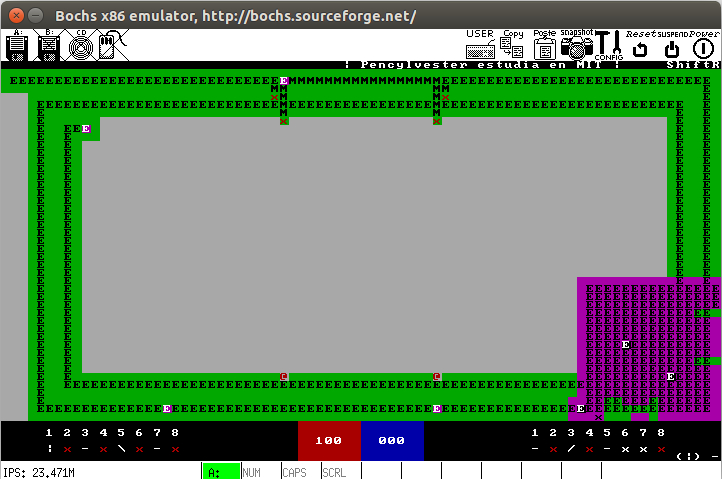
\includegraphics[width=0.7\textwidth]{imagenes/mapa4.png}

Un minero podría
moverse a una posición no descubierta, en cuyo caso tendrá un problema de
{\it page_fault\/} (notar cruces rojas afuera del mapa explorado)
\end{center}

Por último se llama a {\it game_pirata_mover\/} que efectivamente mueve al
pirata. Si se movió correctamente, se devuelve un 0 (ver
{\it game_pirata_mover\/} y {\it game_explorar_posicion\/} en funciones
propias).

\item[game_syscall_cavar] Toma al jugador y al pirata como parámetros y averigua
la posición del pirata, si el pirata es un explorador o no hay monedas
disponibles en esta posicion (botin vacio o no habia botin) se llama a
{\it game_pirata_exploto\/} y se devuelve -1.

En caso contrario, se le suma una moneda al jugador, con {\it game_minar_botin/}
y {\it screen_pintar_puntajes\/}, esta última se encarga de mostrar el nuevo
puntaje en pantalla. Finalmente se devuelve un 0.

\item[game_syscall_pirata_posicion] Recibe por parámetro el {\it jugador\/} y un
{\it index\/}.

Si el index está fuera de rango (menor a -1 o mayor a 7) se mata al pirata y se
devuelve un -1.

Si el index es -1, se apunta al pirata actual, en caso contrario, se apunta a la
posición index del arreglo piratas del jugador pasado por parámetro.

Una vez seleccionado el pirata se devuelve en un solo regsitro la posicion $X$
en los primeros 8 bits y la posicion $Y$ en los siguientes 8, quedando los
últimos 16 sin importancia.

Por último al retornar a la interrupción, esta acomoda la pila, recupera el
parámetro de la interrupción y comprueba si se devolvió un -1
(el pirata explotó), en este caso salta a la tarea idle, en caso contrario, se
fija si se pidió la posición, si fue así, se pone manualmente en la pila en el
registro {\it eax\/} guardado de la tarea la posición actual de la misma, de
manera que al realizarse el {\bf popad} antes de salir de la interrupción se
devuelva la posición en el registro {\it eax\/}.
\end{description}

\subsection{Ejercicio 7}

\begin{itemize}

\item La estructura adoptada para el scheduler, se detalla en la sección {\bf estructuras}.

\item La implementación de sched_proxima_a_ejecutar es como se detalla a
continuación:

  En primer lugar se obtiene el jugador activo, el inactivo y se asigna por defecto
  una variable próximo con valor inicial de 16 (tarea idle). Luego, si el
  scheduler está activo chequea si el jugador inactivo tiene un slot para
  ejecutar, esto lo hace con la funcion {\it sched_hay_slot_a_ejecutar\/}, en esta
  función se recorre la lista de tareas del jugador indicado y si hay una que
  está en ejecución, se devuelve un 1, si no hay ninguna activa, devuelve 0.

  Si esta función retorna un 1, se cambia el jugador actual del scheduler por el
  que se tenía como inactivo y a próximo se le asigna el siguiente slot activo
  de este jugador con la función {\it sched_proximo_slot_a_ejecutar\/}, esta función
  recorre el array de slots del jugador a partir de la ultima tarea ejecutada
  (dando la vuelta y volviendo a la misma si no hay otra) y devolviendo el indice
  de la proxima en la lista que esté en ejecución.

  Si el jugador inactivo no tiene un slot a ejecutar, chequea con
  {\it sched_hay_slot_a_ejecutar\/} lo mismo para el jugador activo y
  también asigna a {\it proximo\/} el índice de la próxima tarea de este jugador a
  ejecutar.

  Si ningún jugador está activo, devuelve {\it proximo\/} con la tarea idle.

\item En {\it sched_tick\/} se llama primero a {\it game_tick\/} que actualiza los
relojes de la pantalla, luego a
  {\it game_mineros_pendientes\/} con el jugador actual del scheduler (se habla más
  de esta función luego) y se define el índice de la próxima tarea a ejecutar
  llamando a {\it sched_proxima_a_ejecutar\/}.

  Finalmente se devuelve el índice de la GDT de la próxima tarea a ejecutar que
  se obtiene del atributo selectores del scheduler con el índice que se consigue
  en el paso anterior. Se modificó también el llamado que hace la interrupción
  del reloj a {\it game_tick\/} por {\it sched_tick\/}.

\item El funcionamiento final de la interrupción $0\times46$ fue detallado en
 la sección del ejercion 6.

\item Se modifico la macro que define el comportamiento de cada interrupcion. la
 única diferencia entre las interrupciones, son las que tienen {\bf error code} y las
  que no. Esto modifica el lugar en la pila de los parámetros que se pasan a la
  función de C {\it game_atender_excepcion\/}, para solucionar esto, se chequea primero
  (de acuerdo a los parámetros pasados a la macro)
  si la excepción genera error code o no, en base a esto se define un {\it offset\/}
  para acceder a la pila y obtener los datos necesarios para luego ponerlos en
  el tope de la pila y llamar a la funcion de C.

  La funcion {\it game_atender_excepcion\/} se encarga de llamar a {\it game_pirata_exploto\/}
  para desalojar el pirata, ademas de chequar si se está en modo debug (con una
  variable global {\it debug\/} que se pone en 0 o en 1) para frenar el scheduler, guardar la
  pantalla actual y mostrar la informacion de debug. de no estar
  en modo debug, vuelve a la interrupción y cambia a la tarea idle.

  \begin{center}
  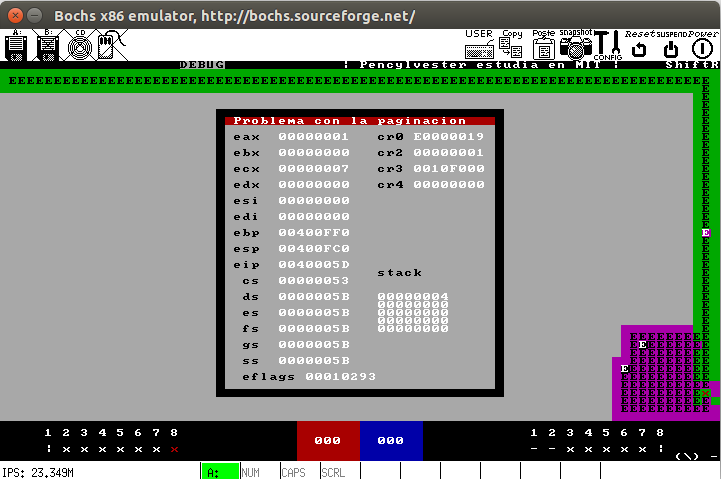
\includegraphics[width=0.7\textwidth]{imagenes/mapa2.png}

  Modo debug
  \end{center}

\item Cuando {\it game_atender_excepcion\/} entra en {\bf modo debug}, realiza lo dicho
anteriormente, guarda la pantalla actual con {\it screen_guardar\/}, imprime lo pedido
por el modo debug con {\it screen_debug\/} la cual toma todos los parámetros que se
pasaron inicialmente por la pila.

\item El modo debug se inicia cuando se llama a la interrupcion del teclado
   presionando la tecla $y$. En este caso se chequea, si ya esta en modo
  debug y se activa el scheduler, continuando la ejecucion del juego.

   En caso de no estarlo, se setea el indicador de debug en 1 lo cual desactivará
  el scheduler cuando haya una excepcion.
\end{itemize}

\section{Estructuras}

\begin{description}
\item[Estructura de paginación del pirata]
  Cada jugador posee un arreglo {\it mapa\/} de 4 posiciones, cuando se
  inicializa el jugador se llama a {\it game_jugador_inicializar_mapa\/}, esta
  función se encarga de pedir por única vez cuatro páginas libres e iniciarlas
  como page tables vacías (todos sus valores a 0), se asigna a las cuatro
  posiciones del arreglo las 4 direcciones de memoria de estas páginas.

  Luego cada pirata tiene su propio page directory con el identity mapping de
  las posiciones del kernel en la primera entrada y su código en la segunda. A
  este page directory también se asignan las 4 posiciones de memoria de las
  tablas que se encuentran en el arreglo mapa de su jugador.

  Cuando un explorador se mueve, este tiene su posicion $X$ e $Y$; con estos valores
  obtiene las posiciones de memoria del mapa a las que se mueve y las mapea en
  este grupo de 4 tablas de paginas, entonces todos los piratas del jugador
  pueden compartir lo explorado por los otros piratas del mismo jugador.

\item[Estructura Jugador]
  La estructura jugador es la encargada de tener la informacion que comparten todos los piratas asi como
  su puntaje, su puerto y donde se encuentra el código de sus tareas.

  La estructura tiene los siguientes atributos:

  \begin{description}
    \item[index] Un identificador (0 para A, 1 para B).
    \item[piratas] Un arreglo de piratas cuya capacidad máxima es el total de
    los que puede tener vivos.
    \item[monedas] La cantidad de monedas que tiene recolectadas
    \item[color] Verde para el jugador A y magenta para el jugador B.
    \item[mapa] Un arreglo de 4 posiciones con las direcciones de memoria de
    las tablas de páginas que se usarán para mapear el mapa visto por sus
    piratas.
    \item[puertoX] Posición $X$ del mapa donde comienza el jugador.
    \item[puertoY] Posición $Y$ del mapa donde comienza el jugador.
    \item[codigo] Las dos direcciones a los códigos de sus piratas, explorador
    en la posición 0 y minero en la posición 1.
    \item[botines] Un arreglo con tantas posiciones como botines hay en el mapa
    el cual sirve para indicar que un botín fue descubierto pero no había slot
    disponible para lanzar un explorador. Una vez se libere un slot, se lanza
    un explorador para el botín descubierto.
  \end{description}

\item[Estructura Pirata]
  La estructura pirata se encarga de conocer a su jugador, su posición actual y
  su tipo.

  Esta tiene los siguientes atributos:

  \begin{description}
    \item[index] Define qué número de pirata es para su jugador.
    \item[jugador] Puntero a su jugador.
    \item[posicionX] Su posición $X$ en el mapa.
    \item[posicionY] Su posición $Y$ en el mapa.
    \item[tipo] Explorador o minero.
  \end{description}

\item[Estructura Scheduler]
  La estructura scheduler es la encargada de saber que tarea está activa en
  este momento y tener la informacion necesaria para saber que tarea ejecutar en
  el próximo ciclo del reloj.

  Esta posee los siguientes atributos:
\begin{description}
    \item[activo] Indica si el scheduler está actualmente manejando el juego o
    no.
    \item[selectores] Este arreglo de 17 posiciones tiene indices a los
    descriptores de las entradas de la GDT de las 8 tareas del jugador A, las 8
    del jugador B y la tarea idle.
    \item[jugadorActual] Como era de esperarse, indica el jugador actualmente
    activo.
    \item[slotActual] Es una tupla que posee el índice del arreglo de slots de
    la última tarea ejecutada por el jugador A en su primer valor, y la última
    del jugador B en su segundo valor.
    \item[slots] Esta tupla de dos arreglos de ocho posiciones indica en cada
    una de ellas si la tarea correspondiente a ese índice (para el jugador A en
    el primer arreglo y el jugador B en el segundo) esta fuera del juego (0) o
    está actualmente en el mapa activa ejecutandosé (1).
\end{description}

\end{description}


\section{Funciones creadas}

\begin{description}
\item[game_mineros_pendientes]
  Esta función chequea si el jugador actual encontró algún botín pero en el
  momento no tenía slots libre para enviar un minero.

  Primero se chequea si el jugador tiene algun slot libre con
  {\it sched_hay_slot_libre\/}, si no lo hay se termina sin hacer nada, si lo
  hay, se cicla el arreglo {\it botín\/} del jugador, el cual indica con un 1 si el
  jugador vió ese botin y no lo envió a minar, o 0 en caso contrario. Si ocurre
   o primero se llama a {\it game_jugador_lanzar_minero\/} con destino al botín
   no minado pero descubierto y se setea a cero la posicion correspondiente del
   arreglo botin del jugador.

\item[game_minar_botin]
  Esta función toma dos parámetros $X$ e $Y$ que indican las coordenadas de una
  posición del mapa.

  Dentro de ella se cicla por el arreglo de botines del mapa y busca el botín
  correspondiente, al que se le resta una moneda y consecuentemente sale del
  ciclo.


\item[game_lineal2virtual] Se encarga de pasar de direcciones lineales del mapa
a las direcciones virtuales correspondientes. Usada para la paginación del mapa.

\item[game_lineal2physical] Se encarga de pasar de direcciones lineales del mapa
a las direcciones físicas correspondientes. Se utiliza para la paginación del
mapa.

\item[game_actualizar_codigo] Esta función toma dos puntos ($X0,Y0$) y ($X1,Y1$)
del mapa.

Con ($X0,Y0$) se obtiene la dirección virtual para esas coordenadas, que es
donde está el código de la tarea actualmente.

Con ($X1,Y1$) obtiene la dirección física en donde se va a pasar el código de
la tarea cuando esta se haya movido. Luego se mapea en la dirección
$0\times400000$ la página física récien obtenida para después copiar desde la
posición actual a la posición $0\times400000$, que apunta a la nueva posición de
la tarea.

\item[game_explorar_posicion]
  Toma como parámetros un puntero a un {\it pirata\/}, un
  {\it page directory\/}, dos puntos $X$ e $Y$ y una dirección.

  En primer lugar se crean 2 arreglos de enteros que representan las coordenadas
  de las posiciones $X$ e $Y$ a mapear.

  Luego se llama a {\it game_calcular_posiciones_vistas\/} con estos dos
  arreglos, las posiciones $X$ e $Y$ que se pasaron en primer lugar, y la
  dirección.
  Esta función devuelve un entero que representa la cantidad de posiciones a
  explorar y asigna en los arreglos dichas posiciones.

  A continuación se recorre con un índice {\it i\/} la cantidad de posiciones,
  se chequea si es una posición válida, si no lo es, no se hace nada
  ; si lo es, se llama a {\it game_pirata_habilitar_posicion\/} que toma como
  parámetro la posición {\it i\/} de los dos arreglos creados en primer lugar y
  el page directory pasado como parámetro a la función principal.

  También se llama a {\it screen_pintar_rect_color\/} con el color del jugador,
  las coordenadas del punto a pintar y 1, 1 (dimensiones del rectángulo a
  pintar).

  Adentro del ciclo también se chequea si la posición tiene botín, si este es el
  caso, se chequea que haya un slot libre, si lo hay, se lanza un minero hacie
  esa posicion; si no lo hay, se escribe un uno en la posición correspondiente a
  este botin en el arreglo {\it botin\/} del jugador correspondiente.

  Por último se pinta en pantalla que hay un botín en esa posición.


\item[game_calcular_posiciones_vistas]
Esta función toma como parámetros dos arreglos, dos enteros que representan una
posición $X$ e $Y$, y una dirección.

Se crean 4 enteros ({\it iniX, iniY\/}), ({\it finX,finY\/}), se comienza un
switch con el parametro {\it dir\/} el cual tiene los siguentes casos:

\begin{lstlisting}
  case IZQ:  iniX = -1; finX = -1; iniY = -1; finY =  1; break;
  case DER:  iniX =  1; finX =  1; iniY = -1; finY =  1; break;
  case ABA:  iniX = -1; finX =  1; iniY =  1; finY =  1; break;
  case ARR:  iniX = -1; finX =  1; iniY = -1; finY = -1; break;
  case TODO: iniX = -1; finX =  1; iniY = -1; finY =  1; break;
\end{lstlisting}

Estos 4 valores indican el lado al que se debe expandir lo explorado
relativamente a la posicion actual, por ejemplo, en el primer caso $X$ comienza
y termina en -1 (lado izquierdo del cuadrado) e Y comienza en -1 y termina en 1
(toda la altura del cuadrado). Entonces luego, con dos ciclos anidados que
recorren estas posiciones relativas de {\it iniX\/} e {\it iniY\/}, se guarda en
los dos arreglos que represetan las posiciones en $X$ y en $Y$ los valores
iniciales de $X$ e $Y$ sumados a este valor relativo, en la posición indicada
por {\it next\/} el cual se va avanzando con cada asignacion, de esta forma en
los arreglos finales se obtienen las nuevas posiciones $X$ e $Y$ que ahora puede
ver el pirata y por ende el jugador.

\begin{center}
\includegraphics[width=0.3\textwidth]{imagenes/habilitarposicion.png}

Posiciones a explorar (verde: posición a la que se mueve)
\end{center}


\item[game_pirata_mover]
  Esta función simplemente llama a {\it game_actualizar_codigo\/} con la
  posición actual del pirata y con otras dos coordenadas, los cuales suelen ser la
  posición a la que el pirata intenta moverse.

  Luego se actualizan los atributos {\it posicionX\/} y {\it posicionY\/} del
  pirata y se llama a {\it screen_pintar_pirata\/} con el pirata modificado, su
  jugador y la dirección.

\item[game_pirata_exploto]
  Esta función pide el pirata actual al {\it scheduler\/}, llama a
  {\it screen_matar_pirata\/}, que lo quita de la pantalla y finalmente llama a
  {\it sched_liberar_slot\/}.

  {\it sched_liberar_slot\/} averigua el jugador actual del scheduler, pide el
  slot de ese jugador y finalmente setea como {\it LIBRE\/} el slot del pirata.

\item[game_calcular_fin]
  Esta función chequea si el contador del juego es igual a la variable global
  FIN, en ese caso se llama a {\it game_terminar_si_es_hora\/} que finaliza el
  juego desactivando el {\it scheduler\/} y el {\it PIC\/} y se devuelve un 1.

  Si el jugo no finalizñó, comprueba si el scheduler está activo y ambos
  jugadores tienen todos los slots ocupados y sus puntajes no cambiaron
  (se usan dos variables globales {\it puntajeA\/} y {\it puntajeB\/} que guardan
  los puntajes de los jugadores en el tick anterior) e incrementa un contador.

  Si algo de esto no se cumple, se resetea el contador y se actualizan las
  variables globales de puntaje de cada jugador. Finalmente se devuelve un 0.

  \begin{center}
  \includegraphics[width=0.7\textwidth]{imagenes/mapa8.png}

  ¡Finish HIM!
  \end{center}

\end{description}
